\documentclass{article}
\usepackage{tikz}
\usetikzlibrary{positioning}
\usetikzlibrary{decorations.markings}
\usepackage[dvipsnames]{xcolor}
\usepackage{amsmath}
\usepackage{pgfplots}
\usepackage{hyperref}
\usepackage{babel}
\usepackage{amssymb}
\hypersetup{
    colorlinks=true,
    linkcolor=blue,
    filecolor=blue,
    urlcolor=blue,
    pdftitle={Matrizen in Neuronalen Netzwerken},
    pdfpagemode=FullScreen,
}
\urlstyle{same}

\begin{document}

\title{Matrizen in Neuronalen Netzen}
\author{Tim Zollner}
\date{17.02.2025}
\maketitle

\newpage

\section{Einleitung}
\glqq Neuronale Netze sind die Kerntechnologie für \textbf{Large Language Models (LLM)}, Anwendungen wie ChatGPT, Technologien aus der \textbf{Bilderkennung} wie Gesichtserkennung und Objekt-Tracking oder \textbf{generative KI} für Bild und Film.\grqq{}(Michael Kipp. Neuronale Netze und Deep Learning. TH Augsburg. \href{https://michaelkipp.de/deeplearning/}{https://michaelkipp.de/deeplearning})

Mithilfe von neuronalen Netzen kann aus einer beliebigen Anzahl an numerischen Eingabewerten (Inputs) ein Ergebnis,
das ebenfalls aus beliebig vielen numerischen Werten besteht berechnet werden.
Diese Berechnung wird durch Parameter, die sogenannten Gewichte und Biases, bestimmt.
Ein Neuronales Netz ist also einfach eine Funktion mit sehr vielen Parametern
Die Berechnung eines Ergebnisses nennt man Feed-Forward, das bestimmen geeigneter Parameter heisst Backpropagation.

\section{Feed-Forward}
\subsection{Einführung}
Bei dem Feed-Forward Prozess wird ausgehend von dem Input $a^0$, also der ersten Schicht, immer die nächste Schicht berechnet.
Dieser Vorgang wird bis zur Ausgabeschicht $a^L$ wiederholt.
Alle Schichten zwischen der Input- und der Ausgabeschicht werden als \glqq Hidden Layer\grqq{} bezeichnet.
Im folgenden Beispiel wäre die Schicht $l=0$ die Eingabeschicht, die Schicht $l=1$ ein \glqq Hidden Layer\grqq{} und die Schicht $l=2$ ($l=L$) die Ausgabeschicht.

\subsection{Grafik}
    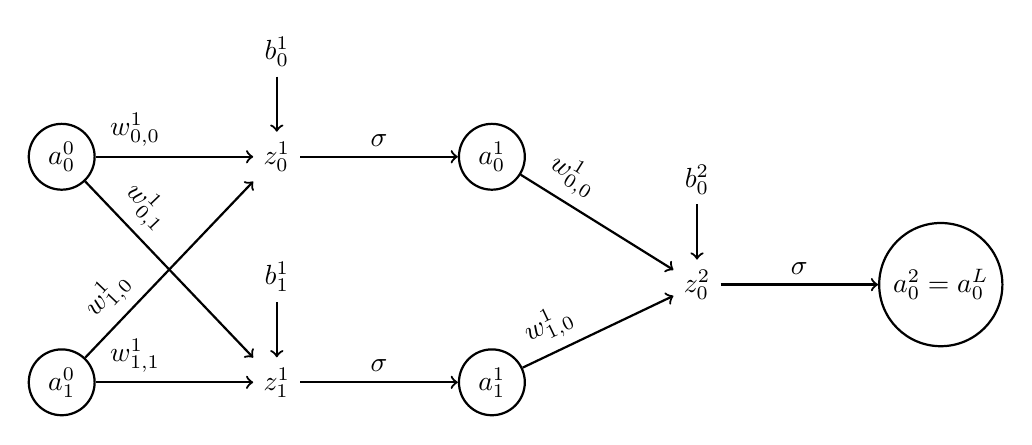
\begin{tikzpicture} [thick, main/.style = {draw, circle}]
        %Knoten
        %\node[main] (z00) {$z_0^0$};
        %\node[main] (z01) [below = 2cm of z00] {$z_1^0$};

        \node[main] (a00)  {$a_0^0$};
        \node[main] (a01) [below = 2cm of a00] {$a_1^0$};

        \node (z10) [right = 2cm of a00] {$z_0^1$};
        \node (z11) [right = 2cm of a01] {$z_1^1$};

        \node (b10) [above = 0.7cm of z10] {$b_0^1$};
        \node (b11) [above = 0.7cm of z11] {$b_1^1$};

        \node[main] (a10) [right = 2cm of z10] {$a_0^1$};
        \node[main] (a11) [right = 2cm of z11] {$a_1^1$};

        \node (z20) [below right = 1cm and 2cm of a10] {$z_0^2$};
        \node (b20) [above = 0.7cm of z20] {$b_0^2$};

        \node[main] (a20) [right = 2cm of z20] {$a_0^2 = a_0^L$};

        %Kanten
        %\draw[->] (z00) -- (a00) node[midway, above] {$\sigma$};
        %\draw[->] (z01) -- (a01) node[midway, above] {$\sigma$};

        \draw[->] (a00) -- (z10) node[pos=0.25, above] {$w_{0,0}^1$};
        \draw[->] (a00) -- (z11) node[pos=0.25, above, sloped] {$w_{0,1}^1$};
        \draw[->] (a01) -- (z10) node[pos=0.25, above, sloped] {$w_{1,0}^1$};
        \draw[->] (a01) -- (z11) node[pos=0.25, above] {$w_{1,1}^1$};

        \draw[->] (b10) -- (z10);
        \draw[->] (b11) -- (z11);

        \draw[->] (z10) -- (a10) node[midway, above] {$\sigma$};
        \draw[->] (z11) -- (a11) node[midway, above] {$\sigma$};


        \draw[->] (a10) -- (z20) node[pos=0.25, above, sloped] {$w_{0,0}^1$};
        \draw[->] (a11) -- (z20) node[pos=0.25, above, sloped] {$w_{1,0}^1$};

        \draw[->] (b20) --(z20);

        \draw[->] (z20) -- (a20) node[midway, above] {$\sigma$};



    \end{tikzpicture}


\subsection{Berechnung}
Dabei ergibt sich der Wert einer Roheingabe aus allen neuronen der vorherigen Schicht.
die Gewichte bestimmen wie viel Einfluss jede vorherige Aktivierung auf den Roheingabe hat. zuletzt wird noch der Bias addiert.

\[ z_0^1 = a_0^0 \cdot \textcolor{OliveGreen}{w_{0,0}} + a_1^0 \cdot \textcolor{OliveGreen}{w_{1,0}} + \textcolor{blue}{b^1} \]
allgemein:
\[  z_i^l = \textcolor{blue}{b_i^l} + \sum_{j=0}^{n^l} a_j^{l-1} \cdot \textcolor{OliveGreen}{w_{j,i}^{l}} \]
Die Roheingabe wir in die Aktivierungsfunktion $\sigma(x)$ eingesetzt um die Aktivierung zu erhalten.
Diese transformiert die Roheingabe zu einem Wert zwischen 0 und 1.
\[ a_j^l = \sigma(z_j^l) 
\kern 40pt
\sigma(x) = \frac{1}{1 + e^{-x}} \]

\subsection{Berechnung als Vektor}
Um die Berechnung der Schichten zu vereinfachen und zu beschleunigen, wird Matrixmultiplikation verwendet.
Dazu werden die gewichte als Matrix, und die Roheingaben, Aktivierungen und Biases einer Schicht jeweils als Vektor behandelt:
\[ \vec{z}^l = \left(\begin{array}{c} z_0^l \\ z_1^l \\ ... \\ z_j^l \end{array}\right) 
\kern 30pt
\vec{a}^l = \left(\begin{array}{c} a_0^l \\ a_1^l \\ ... \\ a_j^l \end{array}\right) 
\kern 30pt
\vec{b}^l = \left(\begin{array}{c} b_0^l \\ b_1^l \\ ... \\ b_j^l \end{array}\right) 
\kern 30pt
W^l = \begin{pmatrix}
    w_{0,0}^l & w_{1,0}^l & ... & w_{j,0}^l \\
    w_{0,1}^l & w_{1,1}^l & ... & w_{j,1}^l \\
    ... & ... & ... & ... \\
    w_{0,i}^l & w_{1,i}^l & ... & w_{j,i}^l
\end{pmatrix} \]
Durch die Matrixmultiplikation fällt das Summenzeichen weg. Außerdem kann eine gesamte Schicht in einem Vorgang berechnet werden

\[ \vec{z}^l = W^l \cdot \vec{a}^{l-1} + \vec{b}^l \]

\[ 
\left(\begin{array}{c} z_0^l \\ z_1^l \\ ... \\ z_i^l \end{array}\right)
=
\begin{pmatrix}
    w_{0,0}^l & w_{1,0}^l & ... & w_{j,0}^l \\
    w_{0,1}^l & w_{1,1}^l & ... & w_{j,1}^l \\
    ... & ... & ... & ... \\
    w_{0,i}^l & w_{1,i}^l & ... & w_{j,i}^l
\end{pmatrix}
\cdot
\left(\begin{array}{c} a_0^{l-1} \\ a_1^{l-1} \\ ... \\ a_j^{l-1} \end{array}\right)
+
\left(\begin{array}{c} b_0^l \\ b_1^l \\ ... \\ b_i^l \end{array}\right)
 \]

 \[
\left(\begin{array}{c} z_0^l \\ z_1^l \\ ... \\ z_i^l \end{array}\right)
=
\left(\begin{array}{c}
    w_{0,0}^l \cdot a_0^{l-1} + w_{1,0}^l \cdot a_1^{l-1} + ... + w_{j,0}^l \cdot a_j^{l-1} \\
    w_{0,1}^l \cdot a_0^{l-1} + w_{1,1}^l \cdot a_1^{l-1} + ... + w_{j,1}^l \cdot a_j^{l-1} \\
    ... \\
    w_{0,i}^l \cdot a_0^{l-1} + w_{1,i}^l \cdot a_1^{l-1} + ... + w_{j,i}^l \cdot a_j^{l-1}
\end{array}\right)
+
\left(\begin{array}{c} b_0^l \\ b_1^l \\ ... \\ b_i^l \end{array}\right)\]


\newpage
\section{Backpropagation}
\subsection{Einführung}
Um die Backpropagation durchführen zu können braucht man zunächst geeignete Trainingsdaten.
Diese bestehen aus Inputdaten und einer gewünschten Ausgabe.
Diese gewünschte Ausgabe wird mit der tatsächlichen Ausgabe der Feed-Forward Berechnung verglichen.
Dann wird jedes Parameter leicht angepasst um das Ergebnis für dieses Beipiel näher an die gewünschte Ausgabe zu bringen.
Durch das Wiederholen mit vielen verschiedenen Trainingsdaten kann eine Parameterbelegung gefunden werden, die für die meisten Inputs ein Ergebnis erzeugt, das dem gewünschten zumindest nahe ist.

\subsection{Verlustfunktion}
Die Verlustfunktion gibt einen numerischen Wert ($E$) für den Unterschied zwischen gewünschter und tatsächlicher Ausgabe aus.
Durch die Potenz werden größere Abweichungen besonders stark gewichtet, während kleinere irrelevant werden.
\[ E_j = \frac{1}{2}(y_j - a_j^L)^2 \]
Bei der Berechnung der Verlustfunktion der gesamten Ausgabeschicht werden die einzelnen Verluste einfach addiert:
\[ E = \frac{1}{2}\sum_{j}^{n^L} (y_j - a_j^L)^2 \]

Die Verlustfunktion ist so gewählt, dass die Ableitung möglichst simpel ist:
\[ \frac{dE_j}{da_{j}^L}  = (a_j^L - y_j) \]


\subsection{Lernvorgang}
Bei dem Lernvorgang wird ein Minimum der Verlustfunktion gesucht.
Da die Verlustfunktion genauso viele Dimensionen wie Parameter hat, ist es unwahrscheinlich, dass man in einem hohen lokalen Minimum \glqq steckenbleibt\grqq{}
Dazu wird die Verlustfunktion nach den einzelnen Parametern abgeleitet um die Steigung der Verlustfunktion zu bestimmen.
Dies wird für mehrere Trainingsbeispiel wiederholt.
Der für die Steigung über mehrere Trainingsbeispiele wird dann von dem anfänglichen Wert des Parameters abgezogen, um die Verlustfunktion zu minimieren.
Dadurch werden Parameter die einen größeren Einfluss auf den finalen Wert der Verlustfunktion haben stärker verändert als andere.
Die Lernrate bestimmt wie start die Parameter bei jedem Durchlauf verändert werden.


\[ w_{j,i}^l \rightarrow w_{j,i}^l - \frac{\eta}{N} \cdot \sum_{k = 0}^{N} \frac{\partial E^k}{\partial w_{j,i}^l} \]
\[ b_j^l \rightarrow b_j^l - \frac{\eta}{N} \cdot \sum_{k = 0}^{N} \frac{\partial E^k}{\partial b_j^l} \]
$\eta$ = Lernrate \kern 20pt $N$ = Anzahl der Trainingsbeispiele \kern 20pt $k$ = Trainingsbeispiel 


\subsection{Ableitung der sigmoid Funktion}
Um nach den Parametern ableiten zu können muss auch die Aktivierungsfunktion abgeleitet werden.
\[ \textcolor{blue}{ \sigma(x) = \frac{1}{1 + e^{-x}} } \]
\[ \textcolor{red}{ \frac{d}{dx}\sigma(x) } = \frac{
0( \cdot 1 + e^{-x}) - 1 \cdot e^{-x} \cdot -1
}{
    (1 + e^{-x})^2
} = \frac{e^{-x}}{(1 + e^{-x})^2} 
= \frac{1 + e^{-x} - 1}{(1 + e^{-x})^2} \]
\[ =\frac{1 + e^{-x}}{(1 + e^{-x})^2} - \frac{1}{(1 + e^{-x})^2} 
= \frac{1}{1 + e^{-x}} - \frac{1}{(1 + e^{-x})^2} \]
\[ = \frac{1}{1 + e^{-x}} \cdot (1 - \frac{1}{1 + e^{-x}}) 
= \textcolor{red}{ \sigma(x) \cdot (1 - \sigma(x)) } \]
Da die Ableitung durch Werte berechnet wird, die bereits im Feed-Forward Prozess bestimmt wurden, können diese wiederverwendet werden.

\resizebox{280pt}{210pt}{
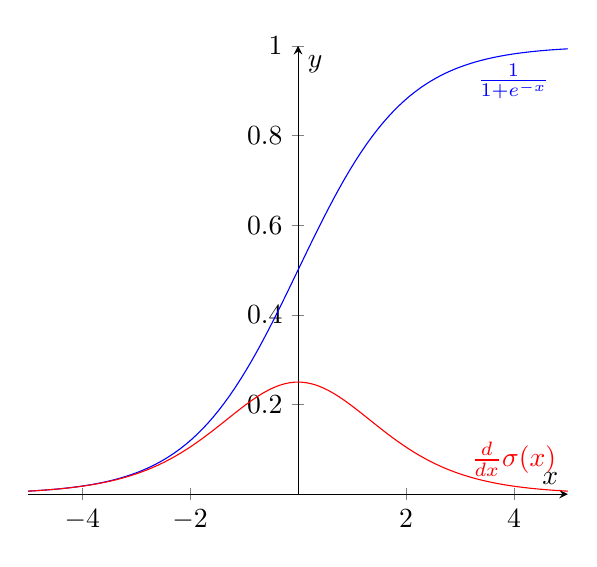
\begin{tikzpicture}[>=stealth]
    \begin{axis}[
        xmin=-5,xmax=5,
        ymin=0,ymax=1,
        axis x line=middle,
        axis y line=middle,
        axis line style=->,
        xlabel={$x$},
        ylabel={$y$},
    ]
    \addplot[no marks, blue] expression[domain=-5:5, samples=100]{1 / (1+ exp(-x))}
    node[pos=0.9, below] {$\frac{1}{1 + e^{-x}}$};
    \addplot[no marks, red] expression[domain=-5:5, samples=100]{1 / (1+ exp(-x)) * (1 - 1 / (1+ exp(-x)))}
    node[pos=0.9, above] {$\frac{d}{dx} \sigma(x)$};

    \end{axis}
\end{tikzpicture}
}

\pagebreak


\subsection{Fehler($\delta$)}
\begin{flushleft}
Der sogenannte Fehler ist ein Zwischenwert der zur berechnung der Änderungsraten der Gewichte und Biases benutzt wird.
Der Fehlerterm berechnet jeweils die partielle Ableitung der Kostenfunktion $E$ nach einer Roheingabe $z$. Es gibt deshalb
für jede Roheingabe einen Fehlerwert.
\end{flushleft}
\[ \delta_j^l = \frac{\partial E}{\partial z_j^l} 
\kern 50pt
 \frac{\partial E}{\partial w_{j,i}^l} = \delta_i^l \cdot a_j^{l-1}
\kern 50pt
\frac{\partial E}{\partial b_j^l} = \delta_j^l \]
\begin{flushleft}
Bei der Berechnung der Fehler wird zunächst die letzte Schicht berechnet und dann rekursiv die anderen Schichten.
Für die Fehler der letzen Schicht ergibt sich durch die Kettenregel die folgende Formel:
\end{flushleft}
\[ \delta_j^L  = \frac{\partial E}{\partial z_j^L}
= \frac{\partial E}{\partial a_j^L} \cdot \frac{\partial a_j^L}{\partial z_j^L}\]
\begin{flushleft}
Nach dem Einsetzen der Ableitungen:
\end{flushleft}
\[ = (a_j^L - y_j) \cdot \sigma (z_j^L) \cdot (1 - \sigma (z_j^L)) \]
\begin{flushleft}
Die Formel für den Fehler der restlichen Schichten kann auf zwei Teile aufgeteilt werden:
\end{flushleft}
\[ \delta_j^{l}  = \frac{\partial E}{\partial z_j^{l}} 
= \textcolor{OliveGreen}{\frac{\partial E}{\partial a_j^{l}}} \cdot \textcolor{blue}{\frac{\partial a_j^{l}}{\partial z_j^{l}}} \]
\begin{flushleft}
    Die Ableitung der Aktivierung nach der Roheingabe entspricht einfach der Ableitung der Aktivierungsfunktion (hier sigmoid):
\end{flushleft}
\[ \textcolor{blue}{\frac{\partial a_j^{l}}{\partial z_j^{l}} = \sigma^{\prime}(z_j^{l})} \]
\begin{flushleft}
    Bei der Berechnung der Ableitung muss der jeweilige Einfluss auf die nachfolgenden Neuronen addiert werden:
\end{flushleft}
\[ \textcolor{OliveGreen}{ \frac{\partial E}{\partial a_j^{l}}} = \sum_{i 
= 0}^{n^{l+1}} \textcolor{Plum}{\frac{\partial E}{\partial z_i^{l+1}}} \cdot \textcolor{red}{\frac{\partial z_i^{l+1}}{\partial a_j^{l}}} 
= \sum_{i = 0}^{n^{l+1}} \textcolor{Plum}{\delta_i^{l+1}} \cdot \textcolor{red}{ \frac{\partial z_i^{l+1}}{\partial a_j^{l}} } \]
\[ \textcolor{red}{ \frac{\partial z_i^{l+1}}{\partial a_j^{l}}
= \frac{\partial}{\partial a_j^{l}} (\sum_{p = 0}^{n^{l+1}} a_p^{l} \cdot w_{p,i}^{l+1} + b_p^{l+1}) = w_{j, i}^{l+1} } \]
\begin{flushleft}
    Die Ableitung der Summe besteht hier aus einem einzigen Gewicht, da die Ableitung $0$ ergibt wenn p $\neq$ j
\end{flushleft}
\[ \textcolor{OliveGreen}{ \frac{\partial E}{\partial a_j^{l}} } = \sum_{i = 0}^{n^{l+1}} \delta_i^{l+1} \cdot \textcolor{red}{ w_{j,i}^{l+1} } \]
\begin{flushleft}
    Nach dem Zusammenführen der Einzelergebnisse ergibt sich die folgende Formel für die Berechnung der Fehlerterme der restlichen Schichten:
\end{flushleft}
\[ \delta_j^{l} = \textcolor{OliveGreen}{[\sum_{i = 0}^{n^{l+1}} \delta_i^{l+1} \cdot w_{j,i}^{l+1} }] \cdot \textcolor{blue}{ \sigma^{\prime}(z_j^{l}) } \]

\subsection{Berechnung des Fehlers als vektor}
Wie bei dem Feed-Forward Prozess, kann auch bei der Backpropagation Matrixmultiplikation eingesetzt werden,
 um die Berechnungen zu vereinfachen und zu beschleunigen

\subsubsection{Fehler des letzten Layers}
Die Berechnung des letzten Layers benutzt noch keine Matrixmultiplikation, da die Parameter die Verlustfunktion nur auf einem direkten weg beeinflussen.
\[ \delta_j^L = (a_j^L - y_j) \cdot \sigma^{\prime} (z_j^L)  \]

\[ \vec{\delta^L} = \left( \begin{array}{c}
     \delta_0^L \\ \delta_1^L \\ ... \\ \delta_j^L 
\end{array} \right)
\kern 30pt
\vec{y} = \left( \begin{array} {c}
    y_0 \\ y_1 \\ ... \\ y_j
\end{array} \right) 
\kern 30pt
\vec{a^L} = \left(\begin{array}{c}
    a_0^L \\ a_1^L \\ ... \\ a_j^L
\end{array} \right) 
\kern 30pt
\vec{z^L} = \left(\begin{array}{c}
    z_0^L \\ z_1^L \\ ... \\ z_j^L
\end{array} \right) 
\]

\[ \vec{\delta^L} = (\vec{a^L} - \vec{y^L}) \odot \sigma^{\prime}(\vec{z^L}) \]


\subsubsection{Definition $\odot$}
Das sogenannte Hadamart Produkt beschreibt die elementweise Multiplikation zweier Vektoren oder Matrizen mit den selben Dimensionen:
\[ \left(\begin{array}{c}
    a_0 \\ a_1 \\ a_2 \\ a_3
\end{array}\right)
\odot \left(\begin{array}{c}
    b_0 \\ b_1 \\ b_2 \\ b_3
\end{array}\right) 
= \left(\begin{array}{c}
    a_0 \cdot b_0 \\ a_1 \cdot b_1 \\ a_2 \cdot b_2 \\ a_3 \cdot b_3
\end{array}\right) \]

\pagebreak
\subsubsection{Fehler eines beliebigen Layers}
Wie beim Feed-Forward Prozess bleibt die Formel, bis auf das wegfallende Summenzeichen, fast gleich. Nur die Gewichtsmatrix muss transponiert werden.
So kann wieder eine gesamte Schicht in einem Vorgang berechnet werden.

\[ \delta_j^{l} = [\sum_{i = 0}^{n^{l+1}} w_{j,i}^{l+1} \cdot \delta_i^{l+1} ] \cdot \sigma^{\prime}(z_j^{l})  \]

\[ \delta_0^l = (\delta_0^{l+1} \cdot \textcolor{red}{w_{0,0}^{l+1}} + \delta_1^{l+1} \cdot \textcolor{red}{w_{0,1}^{l+1}}
 + \textcolor{red}{...} + \delta_i^{l+1} \cdot \textcolor{red}{w_{0,i}^{l+1}}) \cdot \sigma^{\prime}(z_0^{l}) \]

 \[ \delta_1^l = (\delta_0^{l+1} \cdot \textcolor{blue}{w_{1,0}^{l+1}} + \delta_1^{l+1} \cdot \textcolor{blue}{w_{1,1}^{l+1}}
 + \textcolor{blue}{...} + \delta_i^{l+1} \cdot \textcolor{blue}{w_{1,i}^{l+1}}) \cdot \sigma^{\prime}(z_1^{l}) \]

\[ W^{l+1} = \begin{pmatrix}
    \textcolor{red}{w_{0,0}^{l+1}} & \textcolor{blue}{w_{1,0}^{l+1}} & ... & w_{j,0}^{l+1} \\
    \textcolor{red}{w_{0,1}^{l+1}} & \textcolor{blue}{w_{1,1}^{l+1}} & ... & w_{j,1}^{l+1} \\
    \textcolor{red}{...} & \textcolor{blue}{...} & ... & ... \\
    \textcolor{red}{w_{0,i}^{l+1}} & \textcolor{blue}{w_{1,i}^{l+1}} & ... & w_{j,i}^{l+1}
\end{pmatrix} 
\kern 20pt
{(W^{l+1})}^T = \begin{pmatrix}
    \textcolor{red}{w_{0,0}^{l+1}} & \textcolor{red}{w_{0,1}^{l+1}} & \textcolor{red}{...} & \textcolor{red}{w_{0,i}^{l+1}} \\
    \textcolor{blue}{w_{1,0}^{l+1}} & \textcolor{blue}{w_{1,1}^{l+1}} & \textcolor{blue}{...} & \textcolor{blue}{w_{1,i}^{l+1}} \\
    ... & ... & ... & ... \\
    w_{j,0}^{l+1} & w_{j,1}^{l+1} & ... & w_{j,i}^{l+1} 
\end{pmatrix} 
\kern 20pt
\vec{\delta^{l+1}} = \left( \begin{array}{c}
     \delta_0^{l+1} \\ \delta_1^{l+1} \\ ... \\ \delta_j^{l+1} 
\end{array} \right)\]
\[ \Rightarrow \vec{\delta^l} = {(W^{l+1})}^T \cdot \vec{\delta^{l+1}} \odot \sigma^{\prime}(\vec{z^l}) \]


 \subsection{Feed-Forward Berechnung als Matriz}
 In der Vektorberechnung kann der Inputvektor auch durch eine Matrix aus den Inputs mehrerer Trainingbeispiele ersetzt werden.
 Jede Spalte der Matrix enthält die Input-Werte eines Trainingbeispiels.
 Der Bias vektor muss außerdem wie folgt zu einer Matrix umgewandelt werden.
 So wird der Feed-Forward prozess weiter vereinfacht und durch optimierte Matrixmultiplikation beschleunigt.

 \[ A^l = 
 \begin{pmatrix}
    a_0^{l,0} & a_0^{l,1} & ... & a_0^{l,k} \\
    a_1^{l,0} & a_1^{l,1} & ... & a_1^{l,k} \\
    ... & ... & ... & ... \\
    a_j^{l,0} & a_j^{l,1} & ... & a_j^{l,k} \\
 \end{pmatrix}
 \kern 40pt
 B^l = 
  \begin{pmatrix}
    b_0^{l} & b_0^{l} & ... & b_0^{l} \\
    b_1^{l} & b_1^{l} & ... & b_1^{l} \\
    ... & ... & ... & ... \\
    b_j^{l} & b_j^{l} & ... & b_j^{l} \\
 \end{pmatrix} \]



 \[ A^l = \sigma (W^l \cdot A^{[l-1]} + \vec{b^l}) \]



 \subsection{Backpropagation als Matriz}
 Auch bei der Matrixmultiplikation können die Vektoren nach dem selben Prinzip durch Matrizen ersetzt werden.

 \subsubsection{Fehlerberechnung}

 \[ [\delta^l] =
 \begin{pmatrix}
    \delta_0^{l,0} & \delta_0^{l,1} & ... & \delta_0^{l,k} \\
    \delta_1^{l,0} & \delta_1^{l,1} & ... & \delta_1^{l,k} \\
    ... & ... & ... & ... \\
    \delta_j^{l,0} & \delta_j^{l,1} & ... & \delta_j^{l,k} \\
 \end{pmatrix} \]

  \[ [\delta^L] = (Z^L - Y^L) \odot \sigma^{\prime}(A^L) \]
 \[ [\delta^l] = (W^{l+1})^T \cdot [\delta^{l+1}] \odot \sigma^{\prime}(A^l) \]
\[ \Rightarrow  \frac{\partial E}{B^l} = [\delta^l]
\kern 40pt
\Rightarrow  \frac{\partial E}{b_j^l,k} = \delta_j^l,k \]
Um die durchschnittliche Steigung eines Biases zu berechnen, kann man die Bias-Matrix mit einem Einsvektor multiplizieren.
Auch dieser Vorgang wird also durch Matrizen vereinfacht.

\[ \varnothing \frac{E}{b^l} = [\delta^l] \cdot \left(\begin{array}{c}
    1 \\ 1 \\ ... \\ 1
\end{array}\right)
\]




\pagebreak


 \subsubsection{Berechnung der Gradienten der Gewichte}
 %TODO

 \[ [\delta^l] =
 \begin{pmatrix}
    \textcolor{blue}{\delta_0^{l,0}} & \textcolor{blue}{\delta_0^{l,1}} & \textcolor{blue}{...} & \textcolor{blue}{\delta_0^{l,k}} \\
    \delta_1^{l,0} & \delta_1^{l,1} & ... & \delta_1^{l,k} \\
    ... & ... & ... & ... \\
    \delta_j^{l,0} & \delta_j^{l,1} & ... & \delta_j^{l,k} \\
 \end{pmatrix} 
 \kern 30pt
 A^{l-1} = 
 \begin{pmatrix}
    \textcolor{OliveGreen}{a_0^{l-1,0}} & \textcolor{OliveGreen}{a_0^{l-1,1}} & ... & \textcolor{OliveGreen}{a_0^{l-1,k}} \\
    \textcolor{Cyan}{a_1^{l-1,0}} & \textcolor{Cyan}{a_1^{l-1,1}} & \textcolor{Cyan}{...} & \textcolor{Cyan}{a_1^{l-1,k}} \\
    ... & ... & ... & ... \\
    a_j^{l-1,0} & a_j^{l-1,1} & ... & a_j^{l-1,k} \\
 \end{pmatrix} \]

\[ W^l = \begin{pmatrix}
    \textcolor{red}{w_{0,0}^l} & \textcolor{Plum}{w_{1,0}^l} & ... & w_{j,0}^l \\
    w_{0,1}^l & w_{1,1}^l & ... & w_{j,1}^l \\
    ... & ... & ... & ... \\
    w_{0,i}^l & w_{1,i}^l & ... & w_{j,i}^l
\end{pmatrix} \]



 \[ \frac{\partial E^k}{\partial w_{j,i}^{l}} = \delta_i^{l,k} \cdot z_j^{l-1,k} \]
 \[ \textcolor{red}{\frac{\partial E}{\partial w_{0,0}^l}} = 
 \sum_{k = 0}^{N} \textcolor{blue}{\delta_0^{l,k}} \cdot \textcolor{OliveGreen}{a_0^{l-1,k}} \]
  \[ \textcolor{Plum}{\frac{\partial E}{\partial w_{1,0}^l}} = 
 \sum_{k = 0}^{N} \textcolor{blue}{\delta_0^{l,k}} \cdot \textcolor{Cyan}{a_1^{l-1,k}} \]
\[ \Rightarrow \frac{\partial E}{W^l} = [\delta^l] \cdot (A^{l-1})^T \]


\section{Quellen}
\href{http://neuralnetworksanddeeplearning.com}{Michael Nielsen - Neural Networks and Deep Learning}(Algorithmus) \linebreak
\href{https://michaelkipp.de/deeplearning}{Michael Kipp - Neurale Netze und Deep Learning} (Algorithmus) \linebreak
\href{https://sudeepraja.github.io/Neural/}{Sudeep Raja - A Derivation of Backpropagation in Matrix Form} (Prüfen der Batch-weisen Berechnung)

\end{document}